\documentclass[12pt,a4paper]{ctexrep}
\usepackage[a4paper, portrait, margin=0.8in]{geometry}
\usepackage{graphicx} % Required for inserting images
\usepackage{amsmath}
\usepackage{amsfonts}
\usepackage{amssymb}
\usepackage{amsthm}
\usepackage{markdown}
%\usepackage{china2e} 
\usepackage[utf8]{inputenc}
\usepackage{chemarrow}
\usepackage[colorlinks,linkcolor=black]{hyperref}
\usepackage{fancyhdr}

\title{COMP2711H Review}
\author{Based on Lectures from $A.K.Goharshady$. \\ Notes by $Zheng, Siyang$}
\date{December 20, 2024}

\begin{document}
\maketitle

\hypertarget{toc}{}
\tableofcontents


\fancyfoot[R]{\hyperlink{toc}{back to contents}}
\pagestyle{fancy}

\chapter{Propositional logic逻辑学、数论基础}
Proposotional Logic, Predicate Logic and Peano's Axioms, Induction, Well-ordering and Infinite Descent, Induction Problems and Strong Induction.
\section{定义}
\subsection{Operations}
\textbf{Boolean Algebra:}

\begin{tabular}{l l}
Negation: &"$\neg$"\\
Disjunction: &"$\vee$" or logical OR\\
Conjunction: &"$\wedge$" or logical AND\\
Implication: &"$\rightarrow$"\\
XOR: &"$\oplus$" $\rightarrow$ $a\oplus b$ means if $a == b$\\

\end{tabular}

$p \vee (q \wedge r) = (p \vee q) \wedge (p \vee r)$

$p \wedge (q \vee r) = (p \wedge q) \vee (p \wedge r)$

\textbf{Quantifiers:}

Universal quantifier: $\forall$

$\indent$Existential quantifier: $\exists$\\

$\neg \forall x, p(x) \iff \exists x, \neg p(x)$

$\neg \exists x, p(x) \iff \forall x, \neg p(x)$\\

$\forall n,m \in N, n \leq m \iff \exists x \in N, n+x = m$

\subsection{Definitions of 专有名词}
Tantology:恒成立

Predicate:猜想

Proposition:命题

Contradiction:矛盾

\section{公理}
Peano's Axioms:自然数公理 $\rightarrow$ 定义自然数
\section{定理/结论}
$\sqrt 2$ is irrarional. $\leftarrow$ proof by assumpution.

There is infinite amount of prime numbers. $\leftarrow$ proof by assuming finite amount of prime, then $k = \prod_{i=1}^{n}\, p_{i} + 1$, $k = a \times b, a \in \{p_{n}\}$, no infinite descending {$b_{n}$}.\\

\noindent In Fibonnacci numbers, $F_{0} = 0; F_{1} = 1$

$\sum_{i = 1}^{n} F_{i} = F_{n+2}-1$

$\forall n \in N, F_{1}+F_{3}+F_{5}+\dots +F_{2n-1} = F_{2n}-1$

$\forall n \in N, F_{2}+F_{4}+F_{6}+\dots +F_{2n} = F_{2n+1}-1$

$F_{n}$ and $F_{n+1}$ are relatively prime.\\

\noindent $\forall n \geq 1, \, 1^{3}+2^{3}+\dots + n^{3} = (1+2+ \dots +n)^{2}$
\section{重要定理详解}
\noindent Peano's axioms: 

a) 0 is a natural number. 

b) Every natural number has a successor $s(n)$. 

c) For all $n,m \in N$, if $s(n) = s(m)$, then $n = m$. 

d) For every natural number $n$, the successor of n is not 0. 

e) If $K$ is a set such that $0 \in K, \forall n \in N, n \in K \Rightarrow s(n) \in K$, then $K = N$

\noindent "+":

a) $\forall n \in N, n+0 = n$

b) $\forall n,m \in N, n+s(m) = s(n+m)$

\noindent "$\times$":

a) $\forall n, n\times 0 = 0$

b) $\forall n,m \in N, n \times s(m) = n \times m + n$
\section{方法}
\noindent Mathematical induction (数学归纳法): If you want to show $\varphi(n)$ holds for $n \in N$ 

a) Base case: the induction basis holds.($\varphi(0)$ holds)

b) Induction step: when $\varphi(n)$ holds, then $\varphi(n+1)$ holds\\
Strong Induction: proof $\forall n \in N$ , $p(0) \wedge p(1) \wedge \dots \wedge p(n)$ holds $\Rightarrow p(n+1)$.\\
Well-ordering principle: every non-empty subset $A$ of $N$ has a smallest element.\\
Infinite-descent principle: There is no infinite sequence $\{a_{1}, a_{2}, \dots \}$ of natural numbers, such that $\forall i, a_{i} > a_{i+1}$\\
Pigeon-Hole Principle: If we have n holes and n+1 pigeons are put in them, then there exists a hole with at least 2 pigeons.

\chapter{Counting计数, 组合}
Counting, Permutations, Combinations, Balls and Walls, Principle of Inclusion and Exclusion, Generalized Principle of Inclusion and Exclusion, Pigeonhole Principle
\section{定义}
\subsection{Definition of 名词}
Permutations: 排列. [n] = $\{1,2,\dots,n\}$

Onto:单射.

\section{定理/结论}
\subsection{几何意义}
[n] has $2^{n}$ subsets

$\binom{n}{0} + \binom{n}{1} + \binom{n}{2} + \dots + \binom{n}{n} = 2^{n}$

$\sum_{i=0}^{n} (-1)^{n} \binom{n}{i} = 0$ $\Leftarrow$ even sized subsets=odd sized subsets

$n \binom{n-1}{k} = (k+1) \binom{n}{k+1}$ $\Leftarrow$ want to choose k+1 people from n people and designate a captain

$\star \binom{n}{r} = \binom{n-1}{r}+\binom{n-1}{r-1}$ $\Leftarrow$ number of subsets with an arbitrary element + without the element

$\sum_{0\leq j\leq i\leq n} \binom{n}{i}\binom{i}{j} = 3^{n}$ $\Leftarrow$ separate n into 3 parts\\$\indent$
$\binom{n}{r} = \binom{n}{n-r}$
\subsection{结论}
for [n], how many permutations $\pi$ have the property $\forall i, \pi[i] \neq i$ : $d_{n} = (d_{n-1}+d_{n-2})(n-1)$
\subsection{PIE}
Principle of inclusion and exclusion(PIE): Find the whole number of elements in $A_{1} \sim A_{n}$. 

Generalized PIE: Find the number of elements $E(m)$ appearing in exactly $m$ of $A_{1} \sim A_{n}$. 

$\star$经典习题:6 persons, every pair is either friends or enemy.$\Rightarrow$There must exist 3 people who are friends to each other or enemies to each other.
\section{重要定理详解}
\subsection{PIE}
Let $A_{1}, A_{2}, \dots , A_{n}$ be finite sets.

Suppose $x$ is in exactly $r$ of the $n$ sets.

This indicates that $x$ is counted in $\binom{r}{1} \, A_{n}$ s, $\binom{r}{2} \, A_{n_{1}}\cap A_{n_{2}}$ s,$\dots$, $\binom{r}{r} \, A_{n_{1}}\cap A_{n_{2}} \cap \dots \cap A_{n_{r}}$ s.

$\because$ $-\binom{r}{0}+\binom{r}{1}-\binom{r}{2}+\dots+(-1)^{r+1}\binom{r}{r} +\binom{r}{0}= $ number of subsets with odd sizes - number of subsets with even sizes+1 = 1

$\therefore$Set $\omega(t) = \sum_{i_{1},i_{2},\dots,i_{t}}|A_{i_{1}} \cap A_{i_{2}} \cap \dots \cap A_{i_{t}}|$

$\therefore$ \[|\cup_{i=1}^{k} A_{i}| = \sum_{t=1}^{k} (-1)^{t+1} \omega(t)\]

重点在于找$A_{1},A_{2},\dots,A_{n}$!!!\\

\begin{center}
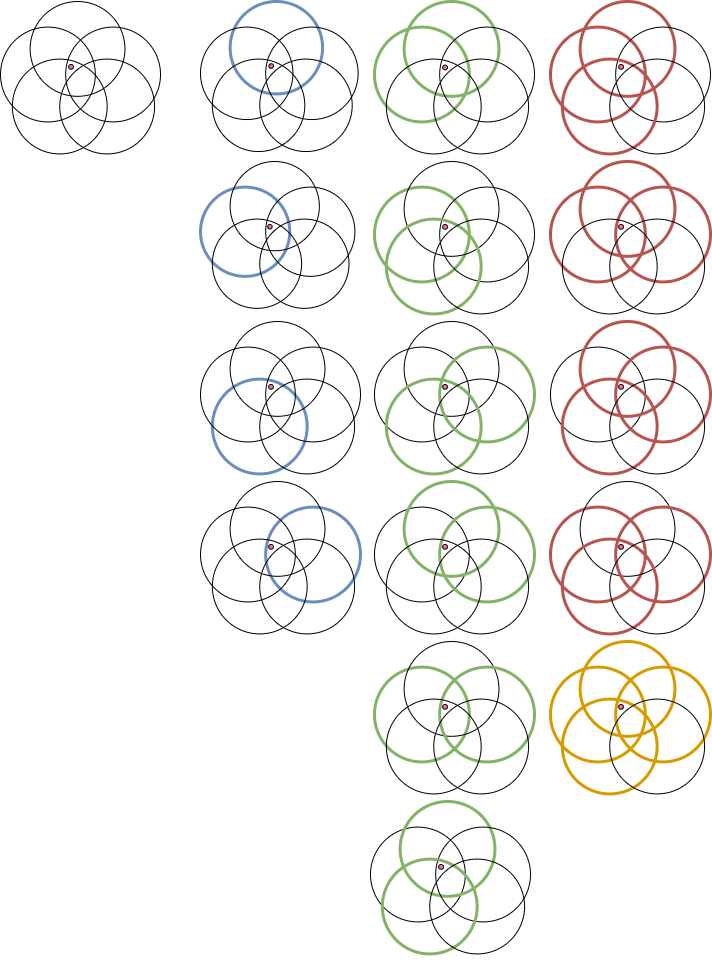
\includegraphics[scale=0.3]{PIE.png}
\end{center}

\subsection{Generalized PIE}
in a universe with n elements, $A_{1}, A_{2}, \dots , A_{n}$ are finite sets.

$\omega(t) = \sum_{i_{1},i_{2},\dots,i_{t}}|A_{i_{1}} \cap A_{i_{2}} \cap \dots \cap A_{i_{t}}|$

$E(m)$ = the number of elements appearing in exactly $m$ of $A_{1} \sim A_{n}$ = \[\sum_{k=m}^{n} (-1)^{k-m} \binom{k}{m} \omega(k)\]

An example are as follows:  \href{https://www.youtube.com/watch?v=D1T3xy_vtxU}{vid}

\begin{center}
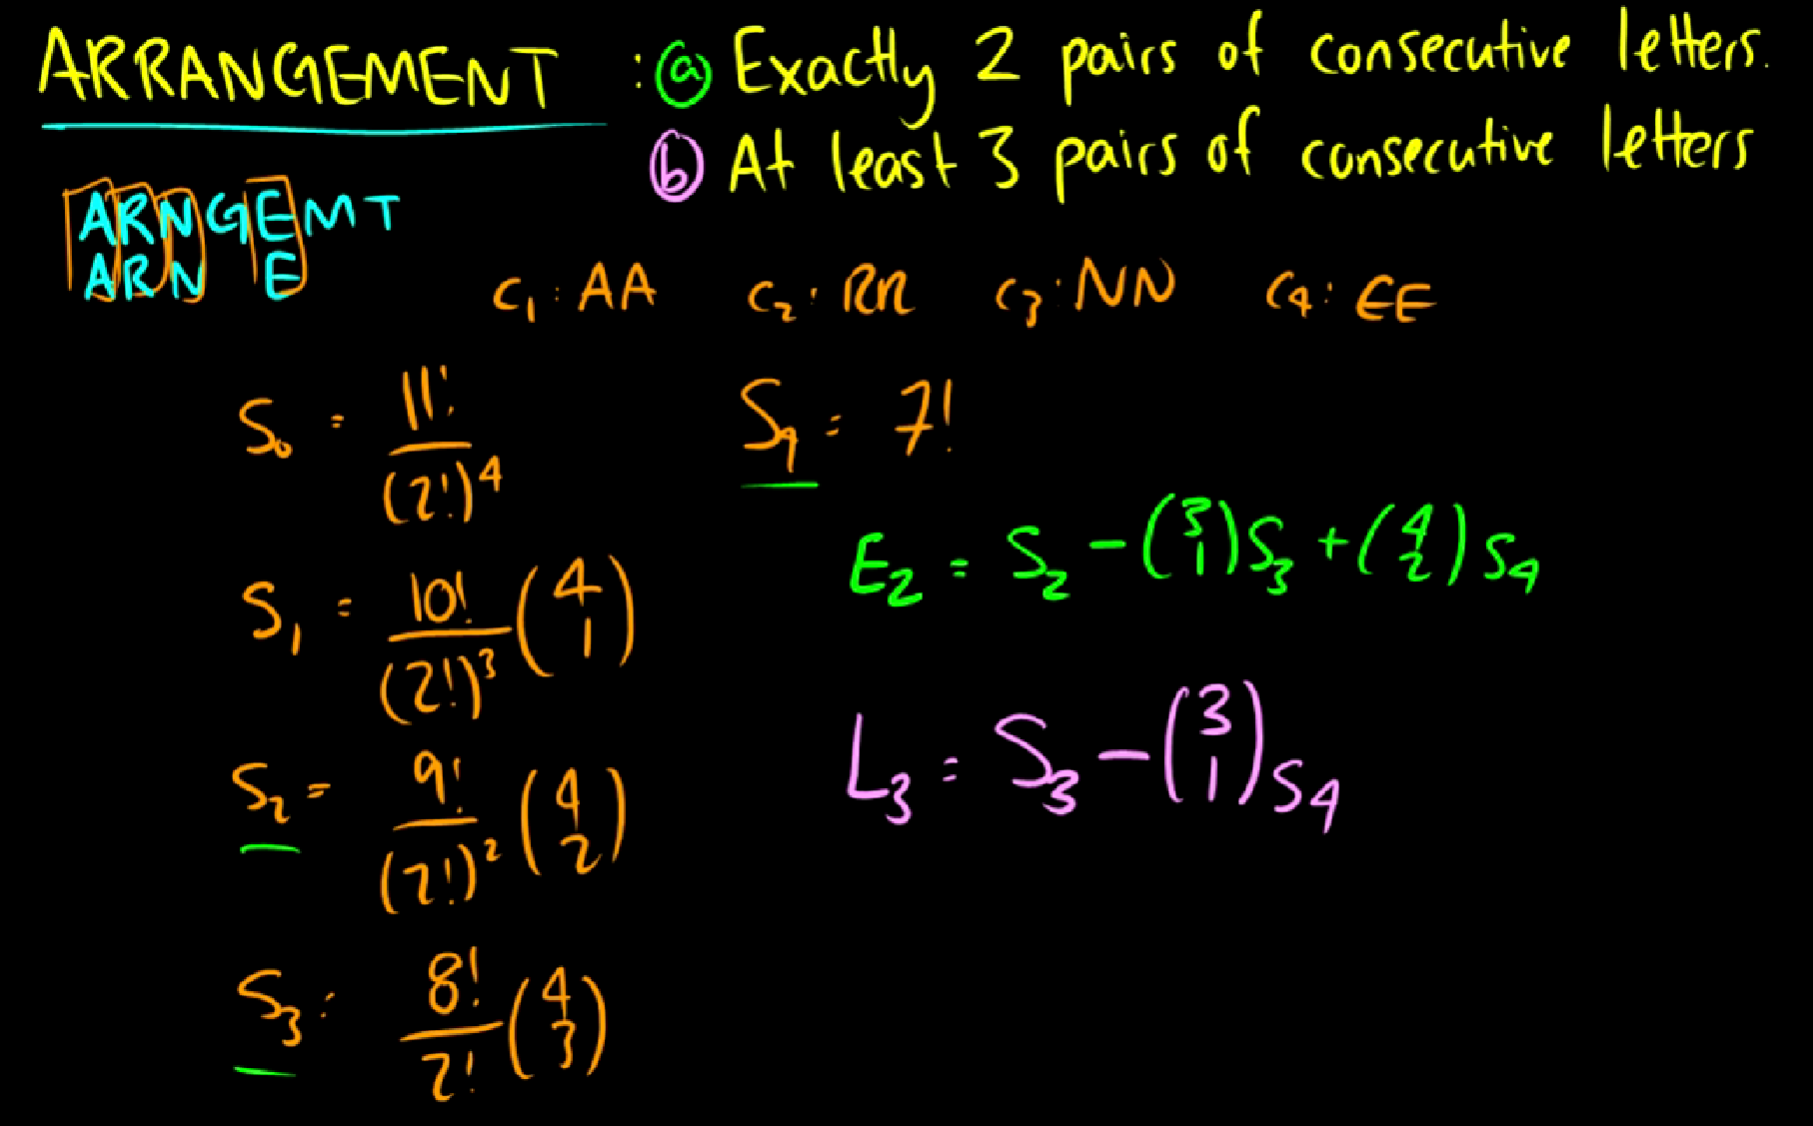
\includegraphics[scale=0.3]{PIE_Example.png}
\end{center}

\section{方法}
Principle of Addition (Case work principle)

Principle of Multiplication

算排列的时候别忘了去重

合理使用induction

插板法

$\indent\star$题目较长的时候,要么用Pigeon-Hole Principle,要么用induction/strong induction

\section{例题}
\subsection{插板法}
How many solutions do we have if $x_1+x_2+x_3+x_4 = 10, x_i \in N$: We have 10 balls and 3 walls, we have $\binom{13}{3}$ solutions.

\subsection{People sitting around circles}
How many ways can $n$ people sit around $r$ circles: 

Let $s(n,r)$ be the ways $n$ people can sit around $r$ circles. Then a person $n$ can sit in his own circle or share a circle with others, therefore $s(n,r) = s(n-1,r-1)+(n-1)s(n-1,r)$.

$\Rightarrow$ if $r=1$, $s(n,1)=(n-1)!$.

\subsection{PIE}
\subsubsection{$n$ students and none of them sit in their chair}
$d_0=1$, $d_1=0$, do induction, when adding a student, let that student sit in $i$'s position, $i$ can sit in $n$'s position, thus $d_{n-2}$, or $i$ can sit in other positions, thus $d_{n-1}$. Therefore, $d_n=d_{n-1}+d_{n-2}$

Extension: How many permutations $\pi$ of $[n]$ have exactly $k$ fixed points? : First select $k$ elements from $n$ elements, then it's a permutation of $n-k$ elements which are not in their own places. Therefore, there's $d_{n,k}=\binom{n}{k} d_{n-k}$

By PIE, let $S_i$ is the number of permutations that has $i$ fixed points, then the number of permutations where no $\pi[i]=i$ is \[d_n=n! - (\sum_{i=1}^n (-1)^{n+1}\binom{n}{i} S_i) = \dots = n! \sum_{i=1}^n \frac{(-1)^{i}}{i!}\]

\subsubsection{How many functions from $[n]$ to $[m]$ are onto}
Number of functions that do not cover the element $i$ in $[m]$ : $|A_i| = (m-1)^n$, then the number of functions that do not cover $k$ elements in $[m]$ are \[S_k = \binom{n}{k} |\cap_{i=a_1,a_2,\dots,a_k} A_i| = \binom{n}{k} (m-k)^n.\] The number of functions that are onto from $[n]$ to $[m]$ are \[O(n,m) = m^n-|\cup_{i=1}^m A_i| = m^n-(\sum_{i=1}^m (-1)^{i+1} S_i = m^n-(\sum_{i=1}^n (-1)^{i+1} \binom{n}{i}(m-i)^n\]

\subsection{PigeonHole Principle}
\subsubsection{choose 10 points from a 3x3 square, there must be two points whose distance < $\sqrt{2}$}
there must be a square of 1x1 where two points are in it, these two points' distance $< \sqrt{2}$
\subsubsection{$\exists x,y \in N, 2024|9^x-9^y$}
$\iff$ $9^x \equiv 9^y$ (mod 2024), because there's only 2024 kinds of remainders when divided by 2024, so when chosen 2025 numbers, there must exist two numbers that has the same remainder.
\subsubsection{There are 6 candidates for president. Every pair of candidates is either friends or enemies. Prove that there are either 3 candidates who are all friends or 3 candidates who are all enemies.}
for a candidate, there's 5 pairs of relations with him, so there must be at least 3 pairs of same relations. Set $A$ is in the same relation with $B,C,D$, if $B,C,D$ are pairwise not in the same relation as $A$, then $B,C,D$ are of the same relation, proofing the assumption. Otherwise, $A$ and the two of them are in the same relation, proofing the assumption.

\chapter{Graph Theory图论}
Graphs, Trees, Paths and Walks, Minimum Spanning Trees, Directed Graphs, DAGs, Tree-based Algorithms and Huffman Coding, Distance, Shortest Paths, Matchings, Vertex Covers, Edge Covers and Independent Sets, Network Flow and the Ford-Fulkerson Algorithm, Stable Matchings and Graph Coloring
\section{定义}
Graph $G = (V,E)$
\subsection{基本名词}
Loop:自环

Neighbors:用一条边连接起来的两点

Complement:补集,$G=(V,E),\,\overline{G}=(V,\overline{E})$

Complete Graph:全集,$K_{n} = (V,E)$, where $\forall u,v \in V, (u,v)\in E$

Degree of a vertex:"度",$d(v)$=number of neighbours of v

Adjacency Matrix:"伴随矩阵", an $n\times n$ matrix where $A_{(i,j)} = 1$ if there's an edge $(i,j)$\\

Walk: a sequence of vertices and edges, vertices and edges can repeat.

Trail: a walk that does not have repeated edges.

Path: a walk that does not have repeated vertices.

Closed walk: a walk that satisfies $v_{0} = v_{n}$.

Cycle: = closed path\\

Connected: Two vertices is connected if they are connected by a path.

Connected Component (CC): a \textbf{maximal} connected subset of vertices.\\

Weights: A functions that maps each edge to a Real number.\\

Distance: $d(u,v) = $number of edges in a $(u,v)$ path.

Eccentricity: $ecc(u) = max\{d(u,v)\},v \in V$

Center: a vertex $u$ is a center of a graph $\iff$ for $\forall v \in V, ecc(u) \leq ecc(v)$

Radius: if $u$ is a center, radius = $ecc(u)$

Diameter: $diam(G) = max\{d(u,v)\},\forall u,v \in V$
\subsection{Tree}
Tree: a connected graph with n-1 edges

Cut: an edge $e \in E$ is a cut $\iff$ $e$ is not part of any cycle. $e$ is a cut if removing it makes the CC it is in into two CC. 

Leaf: a vertex of degree 1.

Spanning Tree:"生成树", A tree that contains every vertex in $G$

Minimum Spanning Tree(MST):"最小生成树", a spanning tree with the least weight.

Rooted Tree: a tree with one vertex chosen as the root. Root at the top and leafs at the bottom.
\subsection{Bipartite}
Bipartite graph: A graph $G=(V,E)$ is bipartite if $V = V_{1}\cup V_{2}$ such that $\forall e \in E$, e has one endpoint in $V_{1}$ and the other endpoint in $V_{2}$
\subsection{Special cycles}
Eulerian circuit: a closed walk that passes over every edge exactly once

Hamiltonian Cycle: a cycle that visits all vertices
\subsection{Graphic}
Graphic: A sequence is graphic if it's the degree of a simple graph.
\subsection{Directed Graph}
Directed Graph: Every $e \in E$ is a $(u,v)$ ordered pair, every vertex has a in-degree and a out-degree.

Strongly Connected(SC): In a directed graph, $u$ and $v$ are strongly connected $\iff$ there's a $(u,v)$-path and a $(v,u)$-path.

Strongly Connected Component(SCC): a \textbf{maximal} connected subset of vertices such that every two vertices is strongly connected.

Directed Acyclic Graphs(DAGs):"有向无环图"

Topological Ordering: In a DAG, a permutation $\pi$ of vertices such that every edge $e\in E$ is of the form $(\pi(i),\pi(j))$,where $i\leq j$. In a topological Ordering, every vertex appear and only appear once, if there's a path $(u,v)$, then, $u$ is in front of $v$
\subsection{Independent Set}
Independent Set: A set $I\subseteq V$, such that for every $e \in E$, $e\notin I$

Maximum Independent Set: The largest possible size of a independent set.
\subsection{Matching}
Matching: A matching $M\subseteq E$ such that no two edges in $M$ share an endpoint.

Maximal Matching: 在维持现状的基础上无法通过再加一条边来增加Matching的数量

Maximum Matching: $\forall M', |M'|<|M|$

Augmenting Path: an alternating path that alternates between $M$ and $E\setminus M$

Number of neighbours: $N(S)$ is the whole number of neighbours of every element in $S$.

Saturate: a Matching $M$ saturates $X$ $\iff$ every vertex $v \in X, v \in M$
\subsection{Vertex Cover $\&$ Edge Cover}
Vertex Cover: a set of vertices such that every edge has at least one endpoint in A.

Minimum Vertex Cover: $\forall VC', |VC'|<|VC|$

Edge Cover: a subset $L\subseteq E$ such that every vertex is incident to at least 1 edge in $L$. ($d(v)\neq 0,v \in V$)
\subsection{Network Flow}
Network: a directed graph $G=(V,E)$, $C:V\times V \rightarrow N$(function Capacity maps every pair of vertices to a Natural number), there's a source($s$) and a sink($t$).

Flow: in a network, $f(u,v)$ is the flow from $u$ directly to $v$. \\
Flow satisfies: 

1.$\forall u,v \in V, f(u,v)\leq C(u,v)$. 

2.$\forall u,v \in V, f(u,v) = -f(v,u)$. 

3.inflow = outflow, $\forall u \in V\setminus \{s,t\} \sum_{v} f(u,v) = \sum_{v} f(v,u) = 0$

$|f| = \sum_{v} f(s,v) = \sum_{v} f(v,t)$

Residual Graph: the graph obtained by subtracting the current flow from the capacity of each edge.
\subsection{Graph Colouring}
Graph Colouring: $k$ colors, a proper colouring is a function $C: V\rightarrow \{1,2,\dots,k\}$, such that for $\forall e \in E$, the two endpoints of $e$ has two different colours.

Chromatic number: $\chi(G)$ is the least number of colours needed to properly colour $G$

$\divideontimes$a bipartite is a graph with $\chi(G)=2$

Clique: $C\subseteq V$ is a clique if $\forall u,v \in C$,$(u,v)$ edge $\in E$,$\omega(G)$= size of the largest clique.即在clique中所有点全连着.

Box Product: Let $G$, $H$ be graphs, $G\Box H =(V_{G} \times V_{H},E_{G \Box H})$

\begin{center}
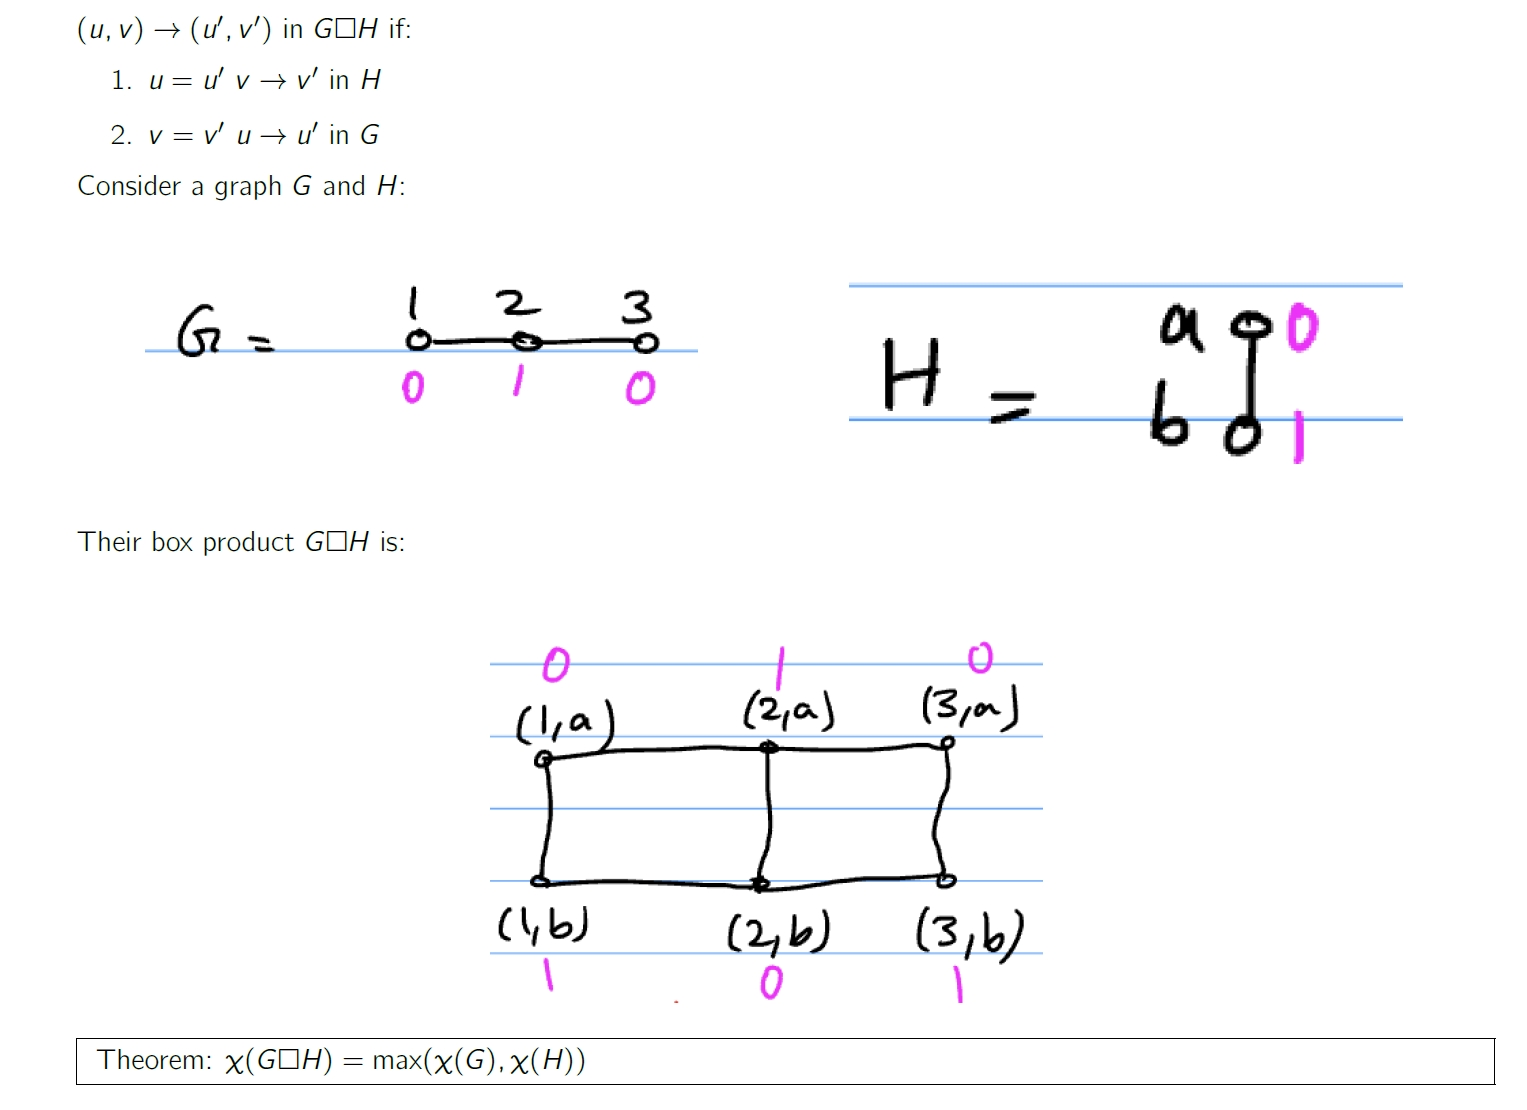
\includegraphics[scale=0.3]{Box_Product.png}
\end{center}
\section{定理/结论}
\subsection{基本结论}
$\sum_{u \in V} d(u) = 2|E|$每多一条边,$\sum d(u)$多二

Every $(u,v)$ walk contains a $(u,v)$ path.

A graph with $n$ vertices and $m$ edges has at least $n-m$ CC

$\Rightarrow$ to connect $n$ vertices, $m \geq n-1$

For $\forall v \in V$, if $d(v)\leq 2$, then $G$ is a cycle or a path.

Every connected graph with $n \geq 2$vertices has $\geq 2$ non-cut vertices.

Every odd closed walk contains an odd cycle.

if $d(i) \geq 2, \forall i \in V$ $\Rightarrow$ G has a cycle.

if $d(i) \leq 2, \forall i \in V$ $\Rightarrow$ G is a cycle or a path.
\subsection{Tree}
Tree's definition: Let $G=(V,E)$, $|V|=n$, $|E|=m$, then \\
"$G$ is connected and $m=n-1$"$\iff$"$G$ is connected and has no cycles"$\iff$ "$m = n-1$, $G$ has no cycles."

$G$ is a tree $\iff$ there is a unique path between every pair of vertices.

A connected graph $G$ is a tree $\iff$ all edges is a cut.

Adding a edge to a tree creates exactly one cycle.

Suppose $V=[n]$, then $2^{\binom{n}{2}}$ graphs exist, and $n^{n-2}$ of them are trees. This is because for every pair of vertices, there can be a edge or not have a edge, so $2^{\binom{n}{2}}$ graphs.

Every connected graph $G$ has a subgraph $T$ such that $T$ is a tree.

If $G$ is a tree, then every longest path in G is a $(u,v)$ path where both $u$ and $v$ are leafs. More about the ways to find the longest path in \ref{sec:Algo_to_longest_path}.

If $T$ is a tree with 3 or more vertices, then no leaf is a center.

Let $T$ be a tree, then $T$ either has 1 center $c$, or 2 neighbouring centers $c_{1},c_{2}$.
\subsection{Bipartite}
A graph is bipartite $\iff$ it has no odd cycle
\subsection{Special Cycles}
$G$ is Eulerian $\iff$ $d(i)$ is even for $\forall i \in V$
\subsection{Graphic}
$d_{1} \sim d_{n}$is graphic $\iff$ $d_{1}-1 \sim d_{n}-1$ is graphic.

$\because$ Every different graphic sequence corresponds to a different tree. $\therefore$ There can be $n^{n-2}$ different trees with $n$ different vertices.
\subsection{Directed Graph}
Let $G$ be a loopless directed graph, $G$ is a DAG $\iff$ $G$ is a SCC.

$G$ is a DAG $\iff$ $G$ has a topological ordering ($G$ has no loops).

In a directed $G$, if the out-degree/in-degree of every vertex is at least 1, then there's a cycle.
\subsection{Matching}
Berge Theorem: A matching $M$ is maximum $\iff$ it does not have an augmenting path.

When $M$ has an augmenting path, then $|M'| = |M|+1$ must exist.

Hall's Theorem: in a XY-bipartite graph, there's a matching $M$ saturating $X$ if and only if for$\forall S \subseteq X, |N(S)|\geq |X|$. More proof in \hyperlink{Hall_proof}{\ref{Hall_proof}}. \label{Hall_theorem}\hypertarget{Hall_theorem}{}

Corollary from Hall's Theorem: Let $G$ be a $k$-regular bipartite graph. ($k$-regular means $d(v) = k,v\in V$)($k\geq 1$).$G$ has a perfect matching.
\subsection{Vertex Cover $\&$ Edge Cover}
In every graph $G$, min $|VC| \geq$ max$|M|$

K\"{o}nig's Theorem: In every bipartite graph $G$, min $|VC|=$ max $|Matching|$.

$A$ is a Vertex Cover $\iff$ $V \setminus A$ is a Independent Set.

In any graph with $|V|=n$, $\max{IS}+\min(VC)=n$

$\max{Matching}+\min{Edge Cover}=n$ for any graph with no isolated vertex.

Gallei's Theorem: In every graph $G$ without isolated vertices, max $|M|$+min$|EC|$=$n$
\subsection{Network Flow}
Max Flow Min Cut Theorem: in a directed graph G, the max flow is the capacity of all the cuts.
\subsection{Stable Matching}
Stable Matching Theorem: In a XY-bipartite graph with sizeof(X)=sizeof(Y)=n, every $x_{i},y_{i}$ has a permutation of Y and X, there's always a stable perfect matching.
\subsection{Graph Colouring}
In every graph $G$, $\chi(G) \geq \omega(G)$, i.e. the color needed to properly color $G$ is greater than the biggest clique.

$chi(G)\geq \frac{n}{\alpha(G)}$. ($\alpha(G)$ is the size of the largest Independent Set.)

Let $G$ be a graph with maximum degree $\delta$, then $\chi(G) \leq 1+\delta$

Brook's Theorem: the only graphs that need $\delta +1$ colours are odd cycles and complete graphs.\

Suppose G is a graph with degree sequence $d_{1}\geq d_{2} \geq d_{3} \geq \dots \geq d_{n}$,then $\chi(G) \leq 1+max_{i}\{min\{d_{i},i-1\}\}$

$\chi(G\Box H)=\max(\chi(G),\chi(H))$
\section{Algorithms}
\subsection{Maximum Spanning Tree}
\subsubsection{Kruskal's algorithm}
sort edges by increasing weight, if choosing the smallest-weight edge that is not in MST creates a cycle, then discard it, if not, then take it into MST.
\subsubsection{Prim's algorithm}
start from any vertex $u$, take the smallest-weight edge from $u \in MST$ to a new vertex not inside MST.

\subsection{Finding the Maximum Independent Set for $G$ is a tree}
pick any arbitrary $v$ as root, let $T_{v}$ be a subtree of $T$ rooted at $v$.

$is_{0}[v] = $the size of the largest IS such that $v \notin I$

$is_{1}[v] = $the size of the largest IS such that $v \in I$

if $l$ is a leaf, then $is_{0}[l] = 0;is_{1}[l] = 1$,

if $l$ isn't a leaf, then $is_{0}[l] = \sum_{c_{i}}(max\{is_{0}[c_{i}], is_{1}[c_{i}]\});\; is_{1}[l] = \sum_{c_{i}}(is_{0}[c_{i}])+1$

output = $max\{is_{0}[r],is_{1}[r]\}$

\subsection{Algorithm to find the longest path} \label{sec:Algo_to_longest_path}
$depth[v] = 1+max\{depth[c_{i},c_{i}$ is $v$'s children$\}$($v$ is not a leaf) or $depth[v] = 0$($v$ is a leaf)

define $lp[v] = $length of the longest path whose highest depth is $v$.

$lp[v] = max\{depth[v],2+max\{c_{i}\}+max\{c_{j}\}\}$($i \neq j$)

\subsection{Path length calculation}
Define $\alpha(u,v,k)$ as 1 if there is a walk with $k$ edges from $u$ to $v$, otherwise 0. then $d(u,v)$ is the smallest $k$ such that $\alpha(u,v,k)=1$.

$\alpha(u,v,k) = \bigvee_{w\in N(v)} \alpha(u,w,k-1)$, $\alpha(u,u,0)=1, \alpha(u,v,0)=0$ for $u \neq v$

\subsection{Dijkastra's Algorithm}
(To find a minimum path from $u$ to $v$ in a non-negative weighted graph)——贪心算法和广度优先的结合

1.从起始点$u$开始计算所有和它相连的点(也就是起始点指向的点),计算完之后把起始点标记下(表示已经计算过了)。

2.找出离起始点最近且没有被标记过的点$v$,计算所有和$v$相连且没有被标记过的点,计算完之后把$v$标记下。即:For each neighbor $n$ of $v$, if($d(u,v)+w(v,n)>d(u,n)$), then update $d(u,w)=d(u,v)+w(v,n)$

3.重复上面的步骤2.直到所有顶点都标记完为止。

\subsection{Ford-Fulkerson's algorithm}
First initialize all $f$ to 0, then find any path from $s$ to $t$ such that every edge in the path is either non-full forward or non-empty backwards. Add to each edge of the path until there's a edge that's empty or full. Repeat.\\

\noindent Greedy Colouring: pick any order for colouring, when colouring vertex $i$, assign the smallest colour number $j$ that's not in its neighbours.
\section{重要定理证明}
\noindent Hall's Theorem:

Theorem in \hyperlink{Hall_theorem}{\ref{Hall_theorem}}. \label{Hall_proof}\hypertarget{Hall_proof}{}.

"$\Rightarrow$": $\because$ It's a matching, $\therefore$ there must be at least one vertex in $Y$ that is a neighbour of a vertex in $X$, $|N(S)|\geq |S|$

"$\Leftarrow$": 取逆否命题,即原命题的反命题:To proof="if maximum matching $M$ does not saturate $X$, then $|N(S)|<|S|$"

$\exists x_{0}\in X, x_{0}\notin M.$ Set $x_{1} \sim x_{n} \in X\cap M = \overline{X}, y_{1} \sim y_{n} \in Y\cap M = \overline{Y}$

a) Proof $x_{0}$'s neighbour is in $\overline{Y}$: if $x_{0}$'s neighbour $\in Y\setminus\overline{Y}$, then count that edge into $M$, contradicting to $x_{0} \notin M$.

b) Proof $\forall x \in \overline{X}, \nexists v\in Y\setminus\overline{Y}$ such that $(x,v)$ is a edge: if so, then $x_{0}, y_{i_{1}}, x_{i_{1}}, y_{i_{2}}, x_{i_{2}}, \dots, y_{i_{n}}, x, v$ is a augmenting path, contradicting to $M$ is a maximum matching.

$\Rightarrow$ $|N(S)| = |\overline{Y}| = |S|-1 < |S|$得证.
\section{方法}
In a game consisting of two players, consider assigning a label to every state of the game.

To proof something exists, construct a algorithm that has a termination proof and a correctness proof.

\chapter{Numbers Theory数论}
Divisibility and Greatest Common Divisor, Prime Factorizations and the Fundamental Theorem of Arithmetic, Congruence, Modular Multiplicative Inverse and the Chinese Remainder Theorem, Fermat's Little Theorem, Euler's Theorem, Wilson's theorem, Diffie-Hellman-Merkle Key Exchange and El-Gamal Encryption, RSA Encryption and Digital Signatures
\section{基本定义}
\paragraph{}
The set of integers:$\mathbb{Z}$ 

Predeccessor, successor

Addition, subtraction, multiplication, absolute value

Division: Let $a,b \in \mathbb{Z}, b>0$, there exist unique $q,r \in \mathbb{Z}$, such that $a=q\times b+r$ and $0\leq r < b$. $a|b$ means there exists integer $x$ that $b = xa$

Greatest Common Divisor(最大公约数): $d|a \wedge d|b$ and $d$ is the greatest.

Relatively prime(互质): $a\perp b \Leftrightarrow gcd(a,b) = 1 \Leftrightarrow \exists x,y \in \mathbb{Z}, ax+by=1$

Least Common Multiple(最小公倍数): $a|l \wedge b|l$ and $l$ is the smallest.

Prime numbers(质数): a integer $p>1$ is prime iff its only divisors are $1,p,-p,-1$

Congruence(同余): $a\equiv b(mod n) \Leftrightarrow n|a-b$. It can be denoted as $a=_n b$

Modular Multiplicative Inverse(MMI): Fixing $n$, $a^{-1}$ is an integer such that $a^{-1}a =_n 1$.

\section{定理/结论}
(Lemma)$\forall a,b \in \mathbb{Z}, b>0$, there exist a $q \in \mathbb{Z}$ such that $q \times b >a$

For $\forall a,b \in \mathbb{Z}$,where $b \neq 0$, there exist unique $q$ and $r$ such that $a = b\times q+r, 0\leq r<b$

Properties of division:
$a|0$, $1|a$, $a|1 \Leftrightarrow a\in \{1,-1\}$, $a|b \wedge c|d \Rightarrow ac|bd$, $a|b \wedge b|c \Rightarrow a|c$, $a|b \wedge b|a \Rightarrow a \in \{b,-b\}$, $a|b \wedge a|c \Rightarrow a|(cx+by)$ for every $x,y$\\

For $\forall a,b \in \mathbb{Z}$, $a,b$ are not both 0, then $\exists x,y \in \mathbb{Z}, gcd(a,b) = ax+by$.

Corollary:
$\forall a,b \in \mathbb{Z}$, $a,b$ are not both 0, $\{ax+by|x,y \in \mathbb{Z}\} = \{q \times gcd(a,b)|q \in \mathbb{Z}\}$

If $gcd(a,b)=d$, then $gcd(\frac{a}{d},\frac{b}{d}) = 1$

If $a|c \wedge b|c$ and $a \perp b$, then $ab|c$

(Euclid's Lemma)
If $a|bc$ and $gcd(a,b) = 1$, then $a|c$

If $a,b \in \mathbb{Z}^+, a = bq+r, 0\leqslant r < b$, then $gcd(a,b) = gcd(b,r) = d$

Let $a,b$ be non-zero positive integers, for negatives, find the absolute value. $gcd(a,b) \times lcm(a,b) = a\times b$

Corollary:
If $a,b$ are positive numbers and they are relatively prime, then $lcm(a,b) = a \times b$

If $p$ is prime and $p|ab$, then $p|a$ or $p|b$ is true.

Corollary:
If $p|a_1a_2\dots a_n$ where $a_i$ is a integer, then, $\exists i$ such that $p|a_i$

Corollary:
If $p|q_1q_2\dots q_n$ where $q_i$ is a prime, then, $\exists i$ such that $p = q_i$

$\bold{F}$undamental $\bold{T}$heorem of $\bold{A}$rithmetic (Prime factorization):
For every integer $n>1$, we can write $n = p_1\times p_2 \times p_3 \times \dots \times p_k$ where every $p_i$ is prime. 存在性,唯一性,对所有$n$都成立\\

There are infinitely many primes.

$a=_nb \iff$ $a$ and $b$ have the same remainders when divided by $n$

Properties of congruences:
$a=_na$, $a=_nb \Leftrightarrow b=_na$, $a=_nb \wedge b=_nc \Rightarrow a=_nc$, $a=_nb \wedge c=_nd \Rightarrow a+b=_nc+d , ab=_ncd$, $a=_nb \Rightarrow ac=_nbc, a+c =_n b+c$, $a+c=_b+c \Rightarrow a=_nb$, $a=_nb \Rightarrow a^k=_nb^k$, $\bold{wrong:}\; ac=_nbc \nRightarrow a=_nb$\\

Applications of MMI:

1.Suppose $ab =_n ac, \, d=gcd(a,n)$, then $ b\equiv c\,(mod\,\frac{n}{d})$

2.Write number $x$ in base $n+1$, the sum of its digits is divisible by $n$ iff the number is divisible by $n$ ($\because n+1 =_n 1$, $\therefore \forall i, (n+1)^i =_n 1^i = 1$, $\therefore x=\sum_{i=0}^j x_i\times(n+1)^i =_n \sum_{i=0}^j x_i$)

Let $P(x)$ be a polynominal function, if $a =_n b$, then $P(a) =_n P(b)$\\

Fermat's Little Theorem:
If $p\nmid a$, then $a^{p-1} =_p 1$ ($p$ is prime)

Euler's totient function:
$\varphi(n) = |\{a|1\leqslant a \leqslant n, a\perp n\}|$. Let $n=\Pi_{i=1}^k {p_i}^{\alpha_i}$, then $\varphi(n) = n\times \Pi_{i=0}^k (1-\frac{1}{p_i})$

Euler's Theorem:
Let $a \perp n$, then $a^{\varphi(n)} =_n 1$

Wilson's Theorem:
For every $p$ ($p$ is prime), $(p-1)! =_p -1$

$\bold{NEED\, TO\, SEE\, HOW\, THEY\, ARE\, PROVED!!!}$

\section{Algorithms算法}
\subsection{Euclidean Algorithm}
To find the greatest common divisor of two numbers:

If $b|a$, then return b, else, $gcd(a,b) = gcd(b,a\%b)$
\subsection{Fast Modular Exponentiation}
To calculate $a^b (mod\, c)$, first write $b$ in base 2, then $a^b =_c a^{b_1} \times a^{b_2} \times \dots \times a^{b_n} =_c a^{b_1}(mod\, c) \times a^{b_2}(mod\, c) \times  \dots \times a^{b_n}(mod\, c)$ where $b_i$ is $2^j$. Calculate iteratively $a^{2^n} (mod\, c)$.

\section{重要定理详解}
\subsection{Infinitely many prime}
Suppose $p_1,p_2,\dots,p_n$ are all the primes, let $q = p_1\times p_2\times \dots \times p_n+1$, then $p_i \nmid q$ for every $p_i$, so $q$ is a prime, contradiction!

\subsection{Modular Multiplicative Inverse} 
For $a,n$, construct a graph $G=(V=[n-1],E=(x,(x+a)\%n))$. If "$a$" and "1" are on the same cycle, then $a^{-1}$ exists.

Proof: $gcd(a,n) = d$, then $d = ax+ny$, $d =_n ax$,$kd =_n kax$, then all multiples of $d$ are on the cycle containing "0", if "1" is on the same cycle, then $\exists x$ such that $ax =_n 1$, $a^{-1} = x$.

$\because$ "1" is on the same cycle as "0" if and only if $gcd(a,n)=1$

$\therefore$ the number $a$ has a mmi $mod\, n$ iff $gcd(a,n)=1$.

\subsection{Chinese Remainder Theorem}
A system of linear congruences: $x =_{n_i} a_i$ where every $n_i$ is relatively prime to each other, have a unique solution. $x-a_i = k_i n_i$, $a_i-a_j = k_in_i-k_jn_j = m_{i,j} \times gcd(n_i,n_j)$, $gcd(n_i,n_j)|a_i-a_j$. 

The solution of $x$ is $x\equiv lcm(a_1,a_2,\dots,a_i) (mod\, n_1n_2\dots n_i)$

Hyperlink: \href{https://youtu.be/EolotL9HN8k?list=PL22w63XsKjqyg3TEfDGsWoMQgWMUMjYhl}{vid}
\subsection{Fermat's Little Theorem}
To proof: $p \nmid a \Rightarrow a^{p-1}=_p 1$ ($p$ is prime)

Let $A=\{a,2a,3a,\dots,(p-1)a\}$, because $p \nmid a$, so $A =_p \{1,2,3,\dots,p-1\}$

Then by multiplying every element in $A$, we have $\prod_{i=1}^{p-1} i\times a =_p 1\times 2\times \dots \times (n-1)$, so $(p-1)!\times a^(p-1) =_p (p-1)!$. By $p\nmid (p-1)!$, we can divide $(p-1)!$ and get the proof to the original Theorem.


\section{Encryption $\&$ Decryption}
\subsection{Symmetric Encryption}
$\overline{m} = Enc(m,key)$ and $m = Dec(\overline{m},key)$
Diffie-Hallman-Merkle key exchange: chooses a very big prime number $p$ and a primitive root $g$ ($\{g^0,g^1,\dots, g^{p-2}\} = \{1,2,3,\dots, p-1\}$ when modulo $p$). Then Alice$\rightarrow$Bob $g^a$ and Bob$\rightarrow$Alice $g^b$, Alice and Bob have a common key $g^{ab} mod\, p$

\subsection{Asymmetric Encryption}
En-Gamal Encryption: Very complicated...%待补充

RSA Encryption:
$e,d \in \{0,1,\dots,n-1\}$, $Enc_e(m) = m^e (mod\, n)$, $Dec_d(\overline{m} = \overline{m}^d (mod\, n)$. Then, $m^{ed} =_p m$, $m^{ed-1} =_p 1$. By Fermat's Little Theorem, $ed =_{p-1} 1$, $d = e^{-1} (mod\, p-1)$. Keygen: pick two large primes $p$ and $q$, calculate and announce $n = p \times q$. Pick $d$, calculate and announce $e = d^{-1} (mod\, lcm(p-1,q-1)$. Only the person knowing $p,q,d$ can decrypt, and anyone knowing $n,e$ can encrypt.

Digital Signature:
Do RSA two times, each with each other's public key.

\chapter{Set Theory集论}
Russell's Paradox and Zermelo–Fraenkel Axioms, Axiom of Infinity and Bijections, Countability and the Theorems of Cantor, Tarski and Schr\"oder–Bernstein, The Set of Real Numbers, $|\mathbb{R}|=|P(\mathbb{N})|$ and the Axiom of Choice
\section{定义}
\subsection{ZFC公理}
\subsubsection{ZF1: Extensionality}
Two sets are equal iff they have the same element.

$(X=Y) \iff (\forall z, z\in X \iff z\in Y)$

\subsubsection{ZF2: Empty Set}
There is a set with no elements.

$\exists X, \forall y, y \notin X$

\subsubsection{ZF3: Unordered Pairs}
If $X$ and $Y$ are sets, there is a set $\{x,y\}$ whose elements are exactly $X$ and $Y$.

$\forall X,Y, \exists Z$ such that $(X \in Z \wedge Y \in Z \wedge(\forall W, W\in Z \Rightarrow (W = X \vee W = Y)))$
%? wikipedia 里没有后面这一串W的
\subsubsection{ZF4: Union}
If $X$ is a set of sets, then there is a set ($A$ in the formula below) consisting of all elements of all elements of $X$.

$\forall X, \exists A, \forall Y,x, (x \in Y\wedge Y \in X \Rightarrow x \in A)$

$A = \cup X = \{x| x\in Y \wedge Y\in X\}$

\subsubsection{ZF5: Comprehension}
If $\varphi(Z,w_1,w_2,\dots,w_n)$ is a formula in $L$ with free variables $Z,w_1,w_2,\dots,w_n$, and $X$ is a set and $a_1,a_2,\dots,a_n$ are sets then $\{y\in X| \varphi(y,a_1,a_2,\dots,a_n)\}$ is a set. 

\subsubsection{ZF6: Powerset}
Let $X$ be a set, there is a set $Y$ whose elements are all subsets of $X$. $Y = \mathbb{P}(X)$

$\forall X, \exists Y, \forall Z : Z \subseteq X \Rightarrow Z \in Y$

\subsubsection{ZF7: Axiom of infinity}
There is a inductive set $\exists X, [\emptyset \in X \wedge (\forall y, y \in X \Rightarrow y \cup \{y\} \in X)] = inductive(X)$

\subsubsection{ZF8: Replacement}
If $\varphi(x,y)$ is a class function and $X$ is a set, then there is a set $Y$ containing exactly $y$s such that $\exists x, \varphi(x,y)$

\subsubsection{ZF9: Foundation}
Every set $X$ contains an $\epsilon$-minimal element.

$\forall x, \exists y, y \in x \wedge x\cap y = \emptyset$

$\forall x, \exists y, y \in x \wedge \forall z \in x \Rightarrow z \notin y$

\subsection{Axiom of Choice}
Every two sets are comparable

1)For every two sets $A$ and $B$, either $|A| \leqslant |B|$ or $|B|\leqslant|A|$

2)For any relation $R$, there's a function $F \subseteq \mathbb{R}$ such that $domain(F) = domain(\mathbb{R})$

3)For every set $A$, there's a function $F: \mathbb{P}(A) \setminus\{\emptyset\} \mapsto A$ such that $\forall B \subseteq A, B \neq \emptyset \Rightarrow F(B) \neq B$

4)For every set $A$ of non-empty disjoint sets, there is a set $C = \cup A$, such that $\forall a \in A, |a\cap C| = 1$

5)Zorn's Lemma: Let $A$ be a set such that for every chain $B \subseteq A$, we have $\cup B \in A$, then $A$ has a maximal element.
\subsection{基本定义}
Ordered Pairs: $\langle x,y\rangle := \{\{x\},\{x,y\}\}$

Class: a collection of the form $X=\{x|\varphi(x)\}$

Cartesian Product: Let $X,Y$ be sets, then $Z = X \times Y = \{\langle x,y\rangle|\forall x\in X, \forall y \in Y\}$. $Z \in \mathbb{P}(\mathbb{P}(X \cup Y))$

Relation: A relation is a subset from $X$ to $Y$: $R\subseteq X\times Y$. Denote it as $X\,R\,Y$

Function: A relation $R \subseteq X \times Y$ is a function $R:X \rightarrow Y$

Successor: If $X$ is a set, $s(X) := X \cup \{X\}$

Inductive: A set is inductive if $0\in X$ and $\forall y \in X \rightarrow s(y) \in X$

Finite Sets: A set $X$ is finite if there is a $N \in \mathbb{N}$ and a function $f:X \rightarrow N$ such that $f$ is one-to-one and onto

Infinite Sets: A set $X$ is infinite if $X$ is not finite.

Cardinality(set的大小): Let $X$ and $Y$ be two sets, then $|X| = |Y|$ or $X\sim Y$ iff there is a bijection $f:X \leftrightarrow Y$. 

Property of Cardinality: 

$\;\forall X, X \sim X$

$\;\forall X,Y,Z, X\sim Y \wedge Y\sim Z \Rightarrow X \sim Z$

$\;\forall X,Y, X\sim Y \Leftrightarrow Y \sim X$

$|X|\leqslant|Y|$ if there exists a one to one function that maps $X$ to $Y$

$\bold{Countable}$: A set is countable if it has the same size as the size of natural numbers. Some examples of countable sets are: the set of even numbers $E$, the set of prime numbers $P$, the set of $k$ natural numbers' Cartesian product $\mathbb{N} \times \mathbb{N} \times \dots\mathbb{N} = \mathbb{N}^k$

Decimal Expansions: 0.$\overline{a_1a_2a_3\dots} = \sum_{i=1} \frac{a_i}{10^i}$\\

Order: Let $A$ be a set. An order on $A$ is a relation $"<"\in A\times A$such that for $\forall a,b \in A$, there are three cases: $a<b,a=b,a>b$ and $\forall a,b,c \in A, a<b \wedge b<c \Rightarrow a<c$

In an ordered set $U$ and $A \subseteq U$,

Upper bound: An element $b \in U$ is an upper bound of $A$ if $\forall a \in A, a \leqslant b$. Let $B$ be all upper bounds of $A$.

Supremum: If there $\exists s \in B$ such that $\forall a \in A, a \leqslant s, \forall s' \in B, s \leqslant s'$. Then $s$ is the supremum of $A$, $s = sup(A)$.

Least Upper Bound Property: If $U$ is an ordered set, then $U$ has the LUB property if every non-empty subset of $U$ \textbf{that has an upper bound}, also has a supremum.

The definition of lower-bound, infimum, largest-lower-bound property is similar.

Dedekind Cut: A cut is a subset $A \subseteq \mathbb{Q}$ such that ($A \neq \mathbb{Q}$ and $A \neq \emptyset$), (If $a \in A$ and $a' \in \mathbb{Q}$ and $a' < a$, then $a' \in A$), ($A$ does not have a maximum).

Define $\mathbb{R} = \{A \subseteq \mathbb{Q}|A$ is a cut$\}$

Define comparison on $\mathbb{R}$: Let $a,b \in \mathbb{R}$, $a \leqslant b \iff a \subseteq b$
Define addition on $\mathbb{R}$: Let $a,b \in \mathbb{R}$, $a+b = \{x+y|x \in a, y \in b\}$

Chain: a set $C$ is a chain if $\forall x,y \in C, x \subseteq y \vee y \subseteq x$
\section{定理/结论}
The empty set is unique.

Let $x,y,a,b$ be sets, $\langle x,y \rangle = \langle a,b \rangle \iff x=a \wedge y=b$

There is a unique set $\mathbb{N}$, such that $\mathbb{N}$ is inductive and for every inductive $X$, we have $X\in \mathbb{N}$

Let $X$ be a set, then $X \notin X$

Let $E$ be the set of even numbers, $|E|=|\mathbb{N}|$: $f:n\mapsto 2n$

Let $P$ be the set of prime numbers, $P=\{p_1,p_2,\dots\}$, $|P|=|\mathbb{N}|$: $f:n \mapsto i$ of $p_i$

$|\mathbb{N} \times \mathbb{N}| = |\mathbb{N}|$

the countable union of countable sets is also countable.

If $A$ is infinite, then $A\setminus \{a\}$ is also infinite.

If $A$ is infinite, then there $\exists X \subseteq A$ such that $|X| = |\mathbb{N}|$

If $A$ is countable and $X$ is infinite, then $A \cup X$ is also countable.\\

Cantor's Theorem:
For every set $A$, $|\mathbb{P}(A)| \neq |A|$ (Proof by contradiction). Proof in \hyperlink{Cantor_proof}{\ref{Cantor_proof}}. \label{Cantor_theorem}\hypertarget{Cantor_theorem}{}

Tarski's Theorem:
%需要进一步解释 %"Btw, I'm not going to give you questions that are this hard in the exams"
Let $X$ be a set. A function $h: \mathbb{P}(X)\mapsto \mathbb{P}(X)$ such that if $A \subseteq B$, then $h(A) \subseteq h(B)$. There exists $C \subseteq X$, such that $h(C)=C$. Proof in \hyperlink{Tarski_proof}{\ref{Tarski_proof}}. \label{Tarski_theorem}\hypertarget{Tarski_theorem}{}

Schr\"odger-Bernstein's Theorem:
If $|X| \leqslant |Y|$ and $|Y| \leqslant |X|$ then $|X| = |Y|$.\\

$0\leqslant x < 1$ is a terminating/ repeating/ mixed decimal expansion, $\iff$ $x$ is a rational number.

If $U$ is an ordered set, then $U$ has the largest-lower-bound property if $U$ also satisfies the least-upper-bound property. This is because for every subset $A$ that is bounded below, $A \neq \emptyset$, so $L = \{x \in U| \forall a \in A, a \geq x\}$. Because $A$ has a lower bound, so $L \neq \emptyset$. By $U$ has the largest-lower-bound property, there exists $\alpha = inf(A)$. It's easy to see that $\alpha$ is also the least-upper-bound of $L$. Therefore, every non-empty subset of $U$ has a least-upper-bound. Proved.

$\mathbb{Q}$ does not have the supremum property, because in $A=\{x \in \mathbb{Q}| x^2<2\}$, $A$ have upper-bounds like 2,3,$\dots$, but the least upper bound does not exist, as $\sqrt{2} \notin \mathbb{Q}$

$\mathbb{R}$ has the supremum property (Least-upper-bound property).

Every number $x\in \mathbb{R}$ has an infinite decimal expansion.

If $a,b,c,d \in \mathbb{R}$, then $|[a,b]| = |(a,b)| = |(a,b]| = |[a,b)| = |[c,d]| = $ infinite.

"Rationals are dense in Reals": $\forall x,y \in \mathbb{R}, x<y \Rightarrow \exists z \in \mathbb{Q} x<z<y$

$|(0,1)| = |(1,+\infty)|$. Proof: $f: x \mapsto \frac{1}{x}$

$|\mathbb{R}| = |(0,1)|$. Proof: $f: (-\infty,-1)\mapsto(0,\frac{1}{3})$, $g: [-1,1]\mapsto[\frac{1}{3},\frac{2}{3}]$, $h: (1,+\infty)\mapsto(\frac{2}{3},1)$

$|\mathbb{R}| = |\mathbb{P}(\mathbb{N})|$

A maximal element of $A$ is an event $m \in A$, such that $\forall a \in A, a \neq m \Rightarrow m \nsubseteq a$
%\section{Algorithms}

\section{重要定理详解}
\subsection{$\mathbb{Q}$ is countable} 
$\mathbb{Q} = \{\frac{a}{b}|(a,b),a \in \mathbb{Z},b\in \mathbb{N}\setminus\{0\},gcd(a,b) = 1\}$. 

$\therefore \mathbb{Q} \subseteq \mathbb{Z}\times \mathbb{N}$

$f: \mathbb{Q}\xrightarrow{1-1}\mathbb{Z}\times\mathbb{N}\autorightarrow{1-1}{onto}\mathbb{N}^2\autorightarrow{1-1}{onto}\mathbb{N}$. $f$ exists, so $|\mathbb{Q}|\leqslant|\mathbb{N}|$

$\because g:\mathbb{N}\mapsto \mathbb{Q}$

$\therefore |\mathbb{N}|\leqslant|\mathbb{Q}|$

$\therefore |\mathbb{Q}| = |\mathbb{N}|$
\subsection{$\mathbb{P}$ is countable}
$f$ takes a finite sequence $a_1,a_2,\dots$, and maps it to $2^{a_1}\times3^{a_2}\times\dots\times p_i^{a_i} \times\dots$. Then, remove the 0s at the end of the sequence, set there are $i$ 0s removed. Let the set of all the finite sequences be $X$, and $\overline{X}$ is the set of all finite sequence with the end 0s removed. By the Arithmetic Fundamental Theorem, $f$ maps $\overline{X}$ to $\mathbb{N}$ and is one-to-one and onto. $g(X) = (i,f(\overline{X}))$, $g:X \mapsto \mathbb{N}^2$ is one-to-one and onto. Therefore $\mathbb{P}$ is countable.

\subsection{Cantor's Theorem}\label{Cantor_proof}
\hyperlink{Cantor_theorem}{\ref{Cantor_theorem}}. \hypertarget{Cantor_proof}{}

Let $g: A \rightarrow \mathbb{P}(A)$ be a bijection. There exists a set $T=\{x \in A| x \notin g(x)\}$, then $T$ is a element in $\mathbb{P}(A)$, i.e. $T \in \mathbb{P}(A)$. Because $g$ is a bijection, there exists $a\in A$ such that $g(a)=T$. For $a$, if $a \in g(a)$, then $a \notin T$, then there's a element in $T$ that is not in $T$, contradiction! If $a \notin g(a)$, then $a \in T$, then there's a element that is not in $T$ is in $T$, contradiction!

\subsection{Tarski's Theorem}\label{Tarski_proof}
\hyperlink{Tarski_theorem}{\ref{Tarski_theorem}}. \hypertarget{Tarski_proof}{}

Let $X$ be a set and $h: \mathbb{P}(X) \rightarrow \mathbb{P}(X)$ be a function such that if $A \in B$ then $h(A) \in h(B)$. Define a set $A \in \mathbb{P}(X)$ is "expansive" if $A \subseteq h(A)$.

Lemma: if $\Omega$ is a set of expansive sets, i.e. $\forall A \in Omega$, $A$ is expansive, then $\bigcup \Omega$ is expansive.

Let $C = \bigcup\{A\in \mathbb{P}(X)| A \subseteq h(A)\}$ be all expansive sets. then by the lemma above, $C$ is also a expansive set, so $h(C)$ exists and $C \subseteq h(C)$. Because by the definition of $h$, $C \in h(C) \Rightarrow h(C) \in h(h(C))$, then $h(C)$ is a expansive set. So $h(C) \in C$, $h(C) = C$.
\section{方法}
\subsection{About sth. that is not countable}
\subsubsection{Vitali Set}
$\mathbb{R}$ is uncountable, $\mathbb{Q}$ is countable $\Rightarrow$ the set of irrational numbers are uncountable.

Define "+" between a (const)number $n$ and a (const)set $A$: $A' = n+A \iff \forall x\in A, x+n \in A' \wedge y \in A', y-n \in A$

We can partition $R$ into uncountably many subsets $V_i$, where each $V_i$ satisfies:

$\forall i,j, \forall a\in V_i, \forall b \in V_j, a \neq b$

$\forall i, \forall a,b \in V_i, a-b \in \mathbb{Q}$

then choose arbitrarily an element from each $V_i$, these elements form a set $V$, $\because |V| = $ the number of $V_i$s $= |$ the number of irrational numbers $|$, $\therefore V $ is uncountable.

\subsubsection{Proof by contradiction}
Let $F = \{f|f:\mathbb{N}\mapsto\{0,1\}\}$,i.e. mapping each $\mathbb{N}$ to every subset of $\mathbb{N}$.

Set $g:\mathbb{N}\mapsto F$ is a bijection, 

there exists a number $t$ where $t[i] = 1-g(i)[i]$, i.e.$\forall i, g(i) \neq t$. Therefore we found a $t \in F$, where no $g$ can map to it. 

\chapter{Probability Theory概率论}
Introduction to Probability Theory, Conditional Probability, Independence and Expectation, Solving Problems using Linearity of Expectation, Markov Chains
\section{定义}
\subsection{基本定义}
Extended Real number: $\mathbb{R}\cup \{-\infty,+\infty\}$. Positive extended reals:$\overline{\mathbb{R}} = [0,+\infty) \cup \{+\infty\}$

Let $A$ be a set and $E \subseteq \mathbb{P}(A)$

Measure: A measure $\mu$ is a function that maps $E$ to $\overline{\mathbb{R}}$

Measure Space: $(A,E,\mu)$. $A$ is the sample space, $E$ is the event space, and $\mu$ is the probability function.

Properties of measure spaces:($\emptyset \in E, \mu(\emptyset) = 0$), (Let $x_1,x_2,x_3\dots \in E$ be countable sets of pairwise disjoint sets, then $\cup_{i=0}^{\infty} x_i\in E, \mu(\cup_{i=0}^{\infty} x_i) = \sum(\cup_{i=0}^{\infty} x_i)$), (if $x \in E$, then $x^C = A \setminus x \in E$)

Lebesque Measure: For every segment from $a$ to $b$, the measure is $(b,a)$. $\mu(\mathbb{R}) = \cup_{i\in \mathbb{Z}} [i,i+1) = \infty$

Probability Space: A probability space $(S,E,Prob)$ is a measure space with total measure 1, i.e. $Prob(S) = 1$. Probability space also satisfies the properties of measure spaces.\\

Conditional Probability: $P(A|B) = \frac{P(A\cap B}{P(B)}$. It's also denoted as $P_B(A)$

Independent events: $A$ and $B$ are independent events if $P(A|B) = P(A)$. Then, they satisfy: $P(AB) = P(A)\times P(B)$

Random Variable: A function $X: S \mapsto \mathbb{R}$. We say $X$ is a discrete random variable if $range(X)$ is either finite or countable

Expectation: $E[X] = \sum_{i = 1}^{\infty} x_i P(X = x_i)$

Stochastic Process: A sequence $x_0,x_1,x_2,\dots$ of random variables.

Markov Chains 见“重要定理详解”
\section{定理/结论}
Linearity of expectation: $A$ and $B$ are two random variables, then $E[aA+B] = aE[A]+E[B]$
\section{重要定理详解}
\subsection{Markov Chain}
Markov Chain: Let $Q$ be a finite set and $\forall i, range(x_i) \subseteq Q$, we say $x_1,x_2,\dots$ is a Markov chain if $\forall n, \forall q \in Q, P(x_n = q_n|x_{n-1} = q_{n-1}) = P(x_n = q_n|x_{n-1} = q_{n-1},x_{n-2} = q_{n-2},\dots,x_{1} = q_{1}$. 即后一项只看前一项,不看再之前的所有项

Markov Chain(Definition using graphs): In $C = (G,\pi,v_0)$ where $G = (V,E)$ is a directed graph, $\pi$ is a function: $E\mapsto [0,1]$ such that for $\forall u \in V, \sum_{v} \pi(u,v) = 1$.($\pi$ is a function that maps all edges to a probability, and the sum of each outgoing edge from a vertex is always 1). Define the probability space $(S,F,P)$, where $S$ is all infinite walks starting from $v_0$, and $F$ is all events, i.e. the extensions of finite paths and anything that can be obtained by their unions/ intersections/ complement. $P$ is the probability function.

Extension: Let $w$ be a finite walk on $G$, then $Ext(w) = \{\overline{w} \in G| \overline{w}$ is an infinite walk with prefix $w\}$

B\"uchi set: There's a target set $T\subseteq V$. $A_i = \{w|w$ is a finite walk on $G$ and exists $i$ $k$s such that all $w[k] \in T\}$. $B_i = Ext(A_i)$. $A_i$ are countable sets, so $B_i$ are countable union of events. $B\ddot{u}chi(T) = \cap_{i=1}^n B_i$ is an event.
%需要继续整理这块

精神状态不正常了:反正就是B\"uchi(v)会无限次的经过v,然后可将一个非Strongly Connected 的graph切分成一堆Strongly Connected Component。在每一个SCC中,一定会有Bottom SCC,即只有ingoing没有outgoing edge。P(最后end up in BSCC) = 1。%这是彩蛋

精神正常后的补充:在一个SCC中,若有一个$v$会被无限次经过,即B\"uchi(v)成立,假设$v'$是$v$的一个successor,那么有限次经过$v'$的概率=$p^n(1-p)^{\infty}$,趋近于0,所以$P(Buchi[v']|Buchi[v])=1$. By conditional probability, $P(Buchi[v'])\geq P(Buchi[v])$. 又因为 $\forall v \in SCC, S=\cup Buchi[v], P(S)=1$,所以肯定有一个$P(Buchi[v])=1$,那么$\forall v \in SCC, P(Buchi[v])=1$。

在一个G中有很多SCC,其中必包含BSCC,那么$P(Buchi[v])$在$v\in BSCC$ 时与上一题相同,而$P(Buchi[v])$在$v \notin BSCC$时=0,因为最后肯定会卡在一个BSCC里,不在BSCC里的点必不会无限次经过

\subsection{Markov decision process}
State space $S$, Action space $A$, State Transitional Probability Matrix $Prob(u,v)$, Reward $Reward(e)$, Discount factor $\gamma$, Policy $Policy(u)$. Refer to an example in Hw4: 

Define function $\bold{EVALUATION}$, input policy at each vertex, and output the modified state values:

For each state $u$, let $v_1,v_2,\dots, v_x$ be all the vertices that $(u,v_i)\in E$, the new state value of $u$ is :\[V(u)=\sum_{i=1}^{x} Policy(u,v_i)\times Prob(u,v_i)\times (Reward(v_i)+\gamma V(v_i))\]. If the new $V(u)$ is very close to the original $V(u)$, then terminate.\\

Define function $\bold{IMPROVE}$, input the policy before and outputs the modified policies:

For each state $u$, let $v_1,v_2,\dots, v_x$ be all the vertices that $(u,v_i)\in E$, set $V(v_m)$ is maximum in all $V(v_i)$, then set $Policy(u,v_m)$ to 1 and all other $Policy(u,v_i)$ to 0. \\

The method is to loop through functions $\bold{EVALUATION}$ and $\bold{IMPROVE}$ again and again. After each time function $\bold{IMPROVE}$ is called, check if the policy before is the same as the policy after modifying. If it's the same, then stop.
%\section{方法}
\section{典型例题}
\subsection{Monty Hall Problem}
有三扇门,其中一扇有奖励,另两个惩罚。玩家先选择一个,然后主持人会打开一个没有奖励的门,此时玩家是否应该换选另一扇仍关着的门?——要换!

Construct a tuple (prize, choice, opened\_door)
\begin{center}
\begin{tabular}{|c|c|c|}
\hline
(1,1,2),(1,1,3) & (1,2,3) & (1,3,2)\\
\hline
(2,1,3) & (2,2,1),(2,2,3) & (2,3,1)\\
\hline
(3,1,2) & (3,2,1) & (3,3,1),(3,3,2)\\
\hline
\end{tabular}
\end{center}
Suppose I chose 1 and the host opens 2, what is the probability of prize in 1? \[P = \frac{P(1,1,2)}{P(1,1,2)+P(3,1,2)} = \frac{1/18}{1/18+1/9} = \frac{1}{3}\]
\subsection{Sleeping Beauty Problem}
玩家在床上睡着了,一个人翻了正常的一枚硬币,如果是正面就把玩家叫醒1次,如果是背面就把玩家叫醒2次。假设玩家无记忆。玩家每次醒来要猜硬币的正反,问玩家猜正还是反赢的概率大?——猜反面!

$E[$正面$] = \frac{1}{2}\times 1 + \frac{1}{2}\times 0 = \frac{1}{2}$

$E[$反面$] = \frac{1}{2}\times 0 + \frac{1}{2}\times 2 = 1$
\subsection{Cancer test}
有一个检测癌症的试纸,如果有癌,则以0.9的概率汇报“+”,如果没癌,则以0.9的概率汇报“-”。假设这个人得癌的概率是p。问得到“+”的汇报有多大概率得了癌症?——$\frac{0.9p}{0.8p+0.1}$

\[P(C|T^+) = \frac{P(C\cap T^+)}{P(T^+)} = \frac{P(T^+|C)P(C)}{P(C)P(T^+|C)+P(C^C)P(T^+|C^C)} = \frac{0.9p}{0.9p+0.1(1-p)} = \frac{0.9p}{0.8p+0.1}\]

\subsection{The Average Number of Times a Coin Needs to Be Flipped Until Head Appears}
有一个正常的硬币,求翻硬币直到翻到为正面向上所需次数的期望。(几何分布Geometric distribution)

法一:Let $X$ be the number of times we need to flip the coin before a Heads appear.

$E[X] = 0.5\times 1 + 0.25\times 2 + \dots + (0.5)^n \times n = 2$

法二:Let $\mu := E[X]$ then $\mu = \frac{1}{2}\times 1 + \frac{1}{2}(1+\mu)$, $\mu = 2$. Explanation: there's a $\frac{1}{2}$ chance of flipping to heads on the first try, and a $\frac{1}{2}$ chance of flipping to tails on the first try and needs a second chance, still with the same expectation.

EXTEND: 改为有一个正面概率为p的硬币:

法一:$E[X'] = \sum_{i=1}^{\infty} (1-p)^{i-1} \times p \times i = \frac{1}{p}$

法二:$E[X'] = p \times 1 + (1-p) \times (1+E[X'])$, Solve the equation, $E[X'] = \frac{1}{p}$

\subsection{Coupon Collector}
一共有n种coupon,每天能随机买一种coupon,问买到所有coupon所需天数的期望

Let $X$ be the number of days we need to collect all coupons. Set $X_i$ as the number of days for going from $i$ coupons to $i+1$ coupons. Then, $X = \sum_{i=0}^{n-1} X_i$, $E(X) = \sum_{i=0}^{n-1} E(X_i)$.

After $i$ types of collected coupons, the next new type of coupon has a $\frac{n-i}{n}$ probability of appearing. So $E(X_i) = \frac{n}{n-i}$. Then $E(X) = \sum_{i=0}^{n-1} \frac{n}{n-i} = n \sum_{i=0}^{n-1}\frac{1}{n-i} = n \sum_{i=1}^{n} \frac{1}{n} = ne$

\chapter{Game Theory游戏论}
Nim and the Sprague-Grundy Theorem, One-shot Games and Nash Equilibria, Two-player Infinite-duration Games on Graphs
\section{定义}
\subsection{基本定义}
Topological Ordering: Given a DAG $G = (V,E)$, a topological ordering is a permutation $\pi$ of vertices such that $\forall e = (u,v)$, the vertex $u$ appears before $v$ in $\pi$.

Dominant Strategy: A strategy $s_i \in S_i$ is dominant if $\forall s_i, u_i(s_i,s_{-i}) \geqslant u_i(s_{i'},s_{-i'})$. A rational player is always going to take the dominant strategy.

Equilibrium State: A state where no one wants to change. (i.e. If only one person changes, then his payoff will decrease)

Nash Equilibrium: Nash Equilibrium is a concept that occurs when each player in a non-cooperative game chooses and stays with their optimal strategy in response to knowing other players' anticipated strategies. Also, no player in a Nash equilibrium has a dominant strategy.

Pure Nash Equilibrium: An outcome $s = (s_1,s_2,\dots)$ is a nash equilibrium iff $\forall i, \forall s'_i, u_i(s_i,s_{-i}) \geqslant u_i(s'_i,s'_{-i})$. Nobody plays randomly in a Pure Nash Equilibrium.

Mixed Nash Equilibrium: Somebody plays randomly, the expectation of other players cannot be increased by playing another strategy.

$\divideontimes$ Nash Equilibrium only applies to games with finite players.\\

Arena: A directed finite graph $G = (V,E,V_1,V_2)$ such that $\forall v \in V$, outdegree($v$)$\geqslant 1$, and $V_1 \cup V_2 = V$, $V_1 \cap V_2 = \emptyset$.

Game: a arena $G = (V,E,V_1,V_2)$ and a starting vertex $v_0\in V$

Strategy: A strategy for player $i$ is a function $\sigma_i = V^* \times V_i \mapsto V$. If the strategy is memoryless, than $V^*$ is  nothing.

Outcome: An outcome is an infinite walk on $G$ starting at $v_0$. $o(\sigma_1)$ is the outcome for the player who uses $\sigma_1$ as his strategy. $O$ is all outcomes of the game.

objective: An objective for player 1 is a set $Obj_1 \subseteq O$.

Zero-Sum game: $Obj_2 = O \setminus Obj_1$

Winning Strategy: A strategy $\sigma_1$ for player 1 is a winning strategy if for $\forall \sigma_2, o(\sigma_1,\sigma_2) \in Obj_1$. The set of initial states from which player i has a winning strategy is $Win_i$.

Determined: A game is determined if for $\forall v_0$ either player 1 or player 2 has a winning strategy.
\section{重要游戏}
\subsection{Nim}
Two numbers, lose if one can't decrease any heap.

Turn-based, finite game, impartial.

We can model these kind of games with directed graphs, where each state in the game corresponds a vertex and a state change corresponds a edge. Assign a "W" or "L" to every vertex. A vertex $v$ is "W" if there's an outgoing edge to "L", but $v$ is "L" if all outgoing edges lead to "W".

Bitwise xor($\oplus$): In base 2, output "1" if the two digits are not the same and output "0" if the two digits are the same. Apply this to every digit of two numbers.

General Nim: We have number $a_1,a_2,\dots,a_n \in \mathbb{N}$ and each player can choose a number and decrease it in their turn. Then $L = \{(a_1,a_2,\dots,a_n)|\oplus_{i=1}^n a_i = 0\}$ and $W = \{(a_1,a_2,\dots,a_n)|\oplus_{i=1}^n a_i \neq 0\}$

\subsection{One-Shot Games}
A one-shot game consists of a set $S_i$ of strategies for each player, a payoff function $u_i: S_i \mapsto \mathbb{R}$. Each player chooses a strategy and the outcome of the game is set. Assume every player is rational, i.e. they choose to maximize their own payoff.
\subsubsection{Prisoner's Dilemma}
\begin{center}
\begin{tabular}{|c|c|c|}
\hline
A  B & Confess & Silent\\
\hline
Confess & 4 4 & 1 5 \\
\hline
Silent & 5 1 & 2 2 \\
\hline

\end{tabular}
Both want to minimize their prison time.
\end{center}
Then both will choose to confess because no matter what the other one choose, confessing gives them the least prison time.

\subsubsection{Pollution Game}
If a country pollutes, then he doesn't cost anything additional, but every country will cost "1". If a country does not pollute, then he will cost "5", and every country else will not cost anything. If everyone is rational, then everyone will pollute.

\section{定理/结论}
Every DAG have a topological ordering.

\subsection{Sprague-Grundy Theorem}
Assign a number to every vertex in $G$: If $v$ has no outgoing edges, then assign $nim(v) = 0$. If $v$ has outgoing edges to $u_1,u_2,\dots,u_n$, then $nim(v) = max\{nim(u_1),nim(u_2),\dots, nim(u_n)\}+1$. Then $L = \{(a_1,a_2,\dots,a_n)|\oplus_{i=1}^n nim(a_i) = 0\}$ and $W = \{(a_1,a_2,\dots,a_n)|\oplus_{i=1}^n nim(a_i) \neq 0\}$

\section{Algorithms}
\subsubsection{Reachability game}
Player 1's objective is to reach $T \subseteq V$

Rule 1: $T \subseteq Win_1$

Rule 2: If $v$ is a player 1 vertex, then $\exists (v,u) \in E, u \in Win_1 \Rightarrow v \in Win_1$

Rule 3: If $v$ is a player 2 vertex, then $\forall (v,u) \in E, u \in Win_1 \Rightarrow v \in Win_1$

This construction algorithm will terminate because there's finite number of vertices, $|Win_1|$ can't increase infinitely.

Process: $T_0 = T$. $T_i = T \cup \{v \in V_1|\exists (v,u)\in E, u \in T_{i-1}\} \cup \{v \in V_2| \forall (v,u)\in E, u \in T_{i-1}\}$

$Win_1$ = $\cup T_i$, denote it as $T_k$

$Win_2$ = $V \setminus Win_1$

Attractor: $Attr_1 = \cup T_i$
\subsection{B\"uchi game}
Player 1's objective is to reach $T \subseteq V$ infinitely many times. 

By "Reachability Game", we are able to find $A_1$ = $Attr_1(T)$(Attracting player 1), $B_1 = A_1^C$(Trapping Player 1), and $C_1 = Attr_2(B_1)$ be the set of vertices that Player 2 can force the game to visit $B_1$, thus trapping Player 1, not letting Player 1 visit $T$ infinitely many times.

Inside $C_1$, Player 2 will not let Player 1 achieve it's goal. Outside $C_1$, for player 1 vertices, player 1 has a outgoing edge that will not enter $C_1$ and will choose it; player 2 does not have a outgoing edge leading to $C_1$ (or it'll be in $C_1$).

Thus, removing $C_1$ part of the whole graph will not affect the final answer to whether player 1 can achieve its goal or not. Remove $C_1$ and we have a smaller game $G_1 = G - C_1$.

Repeat the process using $G_1$ and the same $T$. This process will terminate as $|G|$ is getting smaller every iteration and that $|G|$ is finite.

At the end, $Win_2 = \cup_i C_i$, $Win_1 = V \setminus Win_2$\\

%\begin{figure}
\centering
\includegraphics[scale=0.5]{buchi_game.png}
%\end{figure}
\section{重要定理详解}
%可补充
\end{document}